%% Copernicus Publications Manuscript Preparation Template for LaTeX Submissions
%% ---------------------------------
%% This template should be used for copernicus.cls
%% The class file and some style files are bundled in the Copernicus Latex Package, which can be downloaded from the different journal webpages.
%% For further assistance please contact Copernicus Publications at: production@copernicus.org
%% https://publications.copernicus.org/for_authors/manuscript_preparation.html


%% Please use the following documentclass and journal abbreviations for preprints and final revised papers.

%% 2-column papers and preprints
\documentclass[acp, manuscript]{copernicus}\usepackage[]{graphicx}\usepackage[]{xcolor}
% maxwidth is the original width if it is less than linewidth
% otherwise use linewidth (to make sure the graphics do not exceed the margin)
\makeatletter
\def\maxwidth{ %
  \ifdim\Gin@nat@width>\linewidth
    \linewidth
  \else
    \Gin@nat@width
  \fi
}
\makeatother

\definecolor{fgcolor}{rgb}{0.345, 0.345, 0.345}
\newcommand{\hlnum}[1]{\textcolor[rgb]{0.686,0.059,0.569}{#1}}%
\newcommand{\hlstr}[1]{\textcolor[rgb]{0.192,0.494,0.8}{#1}}%
\newcommand{\hlcom}[1]{\textcolor[rgb]{0.678,0.584,0.686}{\textit{#1}}}%
\newcommand{\hlopt}[1]{\textcolor[rgb]{0,0,0}{#1}}%
\newcommand{\hlstd}[1]{\textcolor[rgb]{0.345,0.345,0.345}{#1}}%
\newcommand{\hlkwa}[1]{\textcolor[rgb]{0.161,0.373,0.58}{\textbf{#1}}}%
\newcommand{\hlkwb}[1]{\textcolor[rgb]{0.69,0.353,0.396}{#1}}%
\newcommand{\hlkwc}[1]{\textcolor[rgb]{0.333,0.667,0.333}{#1}}%
\newcommand{\hlkwd}[1]{\textcolor[rgb]{0.737,0.353,0.396}{\textbf{#1}}}%
\let\hlipl\hlkwb

\usepackage{framed}
\makeatletter
\newenvironment{kframe}{%
 \def\at@end@of@kframe{}%
 \ifinner\ifhmode%
  \def\at@end@of@kframe{\end{minipage}}%
  \begin{minipage}{\columnwidth}%
 \fi\fi%
 \def\FrameCommand##1{\hskip\@totalleftmargin \hskip-\fboxsep
 \colorbox{shadecolor}{##1}\hskip-\fboxsep
     % There is no \\@totalrightmargin, so:
     \hskip-\linewidth \hskip-\@totalleftmargin \hskip\columnwidth}%
 \MakeFramed {\advance\hsize-\width
   \@totalleftmargin\z@ \linewidth\hsize
   \@setminipage}}%
 {\par\unskip\endMakeFramed%
 \at@end@of@kframe}
\makeatother

\definecolor{shadecolor}{rgb}{.97, .97, .97}
\definecolor{messagecolor}{rgb}{0, 0, 0}
\definecolor{warningcolor}{rgb}{1, 0, 1}
\definecolor{errorcolor}{rgb}{1, 0, 0}
\newenvironment{knitrout}{}{} % an empty environment to be redefined in TeX

\usepackage{alltt}



%% Journal abbreviations (please use the same for preprints and final revised papers)


% Advances in Geosciences (adgeo)
% Advances in Radio Science (ars)
% Advances in Science and Research (asr)
% Advances in Statistical Climatology, Meteorology and Oceanography (ascmo)
% Annales Geophysicae (angeo)
% Archives Animal Breeding (aab)
% Atmospheric Chemistry and Physics (acp)
% Atmospheric Measurement Techniques (amt)
% Biogeosciences (bg)
% Climate of the Past (cp)
% DEUQUA Special Publications (deuquasp)
% Drinking Water Engineering and Science (dwes)
% Earth Surface Dynamics (esurf)
% Earth System Dynamics (esd)
% Earth System Science Data (essd)
% E&G Quaternary Science Journal (egqsj)
% EGUsphere (egusphere) | This is only for EGUsphere preprints submitted without relation to an EGU journal.
% European Journal of Mineralogy (ejm)
% Fossil Record (fr)
% Geochronology (gchron)
% Geographica Helvetica (gh)
% Geoscience Communication (gc)
% Geoscientific Instrumentation, Methods and Data Systems (gi)
% Geoscientific Model Development (gmd)
% History of Geo- and Space Sciences (hgss)
% Hydrology and Earth System Sciences (hess)
% Journal of Bone and Joint Infection (jbji)
% Journal of Micropalaeontology (jm)
% Journal of Sensors and Sensor Systems (jsss)
% Magnetic Resonance (mr)
% Mechanical Sciences (ms)
% Natural Hazards and Earth System Sciences (nhess)
% Nonlinear Processes in Geophysics (npg)
% Ocean Science (os)
% Polarforschung - Journal of the German Society for Polar Research (polf)
% Primate Biology (pb)
% Proceedings of the International Association of Hydrological Sciences (piahs)
% Safety of Nuclear Waste Disposal (sand)
% Scientific Drilling (sd)
% SOIL (soil)
% Solid Earth (se)
% The Cryosphere (tc)
% Weather and Climate Dynamics (wcd)
% Web Ecology (we)
% Wind Energy Science (wes)


%% \usepackage commands included in the copernicus.cls:
%\usepackage[german, english]{babel}
%\usepackage{tabularx}
%\usepackage{cancel}
%\usepackage{multirow}
%\usepackage{supertabular}
%\usepackage{algorithmic}
%\usepackage{algorithm}
%\usepackage{amsthm}
%\usepackage{float}
%\usepackage{subfig}
%\usepackage{rotating}
\usepackage{newtxmath}
\usepackage{soul}

\usepackage{todonotes}
\newcommand{\jmu}{\ensuremath{j_\mu}}
\newcommand{\jmcomment}[1]{\todo[inline, color=red!50]{\jmu: #1}}
\newcommand{\egcomment}[1]{\todo[inline, color=brown!50]{\textbf{eg}: #1}}
\newcommand{\yzcomment}[1]{\todo[inline, color=yellow!50]{\textbf{yz}: #1}}
\newcommand{\jqcomment}[1]{\todo[inline, color=blue!50]{\textbf{jq}: #1}}
\newcommand{\avcomment}[1]{\todo[inline, color=green!40]{\textbf{av}: #1}}
\newcommand{\hwcomment}[1]{\todo[inline, color=brown!50]{\textbf{hw}: #1}}
\newcommand{\dscomment}[1]{\todo[inline, color=purple!50]{\textbf{ds}: #1}}
\newcommand{\mccomment}[1]{\todo[inline, color=orange!40]{\textbf{mc}: #1}}
\newcommand{\agcomment}[1]{\todo[inline, color=cyan!40]{\textbf{AG}: #1}}
\newcommand{\afcomment}[1]{\todo[inline, color=grey!40]{\textbf{af}: #1}}
\newcommand{\pscomment}[1]{\todo[inline, color=orange!40]{\textbf{ps}: #1}}

\newcommand{\omegaf}{\ensuremath{\omega_{500}}}
\renewcommand\d[2]{\ensuremath{\frac{d#1}{d#2}}}
\newcommand\dd[2]{\ensuremath{\frac{\partial#1}{\partial#2}}}
\newcommand\D[2]{\ensuremath{\frac{D#1}{D#2}}}
\newcommand\ddp[2]{\ensuremath{\partial#1/\partial#2}}
\newcommand\DDP[2]{\ensuremath{D#1/D#2}}
\newcommand\erfaci{ERF$_\text{aci}$}
\newcommand\erfaer{ERF$_\text{aer}$}
%% \newcommand\degree{\ensuremath{{}^\circ}}
\newcommand\cor{\ensuremath{\text{cor}}}
\newcommand\nd{\ensuremath{N_d}}
\renewcommand\ni{\ensuremath{N_i}} %% replaces "not in" set operator
\newcommand\cdnc{\nd}
\newcommand\lwp{\ensuremath{\mathcal L}}
\newcommand\iwp{\ensuremath{\mathcal I}}
\newcommand\twp{\ensuremath{\mathcal L} + \ensuremath{\mathcal I}}
\newcommand\fc{\ensuremath{f_c}}
\newcommand\cf{\fc}
\newcommand\re{\ensuremath{r_e}}

\newcommand\ql{\ensuremath{q_l}}
\newcommand\qi{\ensuremath{q_i}}
\newcommand\phase{\ensuremath{\varphi}}

\newcommand\swcre{\ensuremath{\mathcal{S}_c}}

\newcommand\fboptics{\ensuremath{\lambda_\text{o}}}
\newcommand\fblifetime{\ensuremath{\lambda_\ell}}
\newcommand\fbphase{\ensuremath{\lambda_{\phase}}}
\newcommand\fbtwp{\ensuremath{\lambda_{\twp}}}

\newcommand\lon{\ensuremath{\lambda}}
\newcommand\lat{\ensuremath{\phi}}
















\IfFileExists{upquote.sty}{\usepackage{upquote}}{}
\begin{document}

\title{General circulation models simulate negative liquid water path--droplet
  number correlations, but anthropogenic aerosols still increase
  simulated liquid water path}


% \Author[affil]{given_name}{surname}

\Author[1]{Johannes}{M\"ulmenst\"adt}
\Author[2]{Edward}{Gryspeerdt}
\Author[3]{S.}{Dipu}
\Author[3]{Johannes}{Quaas}
\Author[4]{Andrew S.}{Ackerman}
\Author[4]{Ann M.}{Fridlind}
\Author[4,5]{Florian}{Tornow}
\Author[4]{Susanne E.}{Bauer}
\Author[1]{Andrew}{Gettelman}
\Author[6]{Yi}{Ming}
\Author[7,8]{Youtong}{Zheng}
\Author[1]{Po-Lun}{Ma}
\Author[1]{Hailong}{Wang}
\Author[1]{Kai}{Zhang}
\Author[1]{Matthew W.}{Christensen}
\Author[1]{Adam C.}{Varble}
\Author[1]{L.~Ruby}{Leung}
\Author[9]{Xiaohong}{Liu}
\Author[10]{David}{Neubauer}
\Author[11]{Daniel G.}{Partridge}
\Author[12]{Philip}{Stier}
\Author[13]{Toshihiko}{Takemura}
\affil[1]{Atmospheric, Climate and Earth Sciences Division, Pacific Northwest
  National Laboratory, Richland, WA, USA}
\affil[2]{Grantham Institute - Climate Change and the Environment, Imperial
  College London, UK}
\affil[3]{Leipzig Institute for Meteorology, Leipzig University, Leipzig, Germany}
\affil[4]{NASA Goddard Institute for Space Studies, New York, NY, USA}
\affil[5]{Columbia University Center for Climate System Research, New York, NY, USA}
\affil[6]{Boston College, Boston, MA, USA}
\affil[7]{Atmospheric and Oceanic Science Program, Princeton University,
  Princeton, NJ, USA}
\affil[8]{Department of Earth and Atmospheric Science, University of Houston,
  Houston, TX, USA}
\affil[9]{Texas A\&M University, College Station, TX, USA}
\affil[10]{Institute for Atmospheric and Climate Science, ETH Z\"urich, Zurich, Switzerland}
\affil[11]{Department of Mathematics and Statistics, University of Exeter, UK}
\affil[12]{Atmospheric, Oceanic and Planetary Physics, Department of Physics, University of Oxford, UK}
\affil[13]{Research Institute for Applied Mechanics, Kyushu University, Fukuoka, Japan}

%% The [] brackets identify the author with the corresponding affiliation. 1, 2, 3, etc. should be inserted.

%% If an author is deceased, please mark the respective author name(s) with a dagger, e.g. "\Author[2,$\dag$]{Anton}{Smith}", and add a further "\affil[$\dag$]{deceased, 1 July 2019}".

%% If authors contributed equally, please mark the respective author names with an asterisk, e.g. "\Author[2,*]{Anton}{Smith}" and "\Author[3,*]{Bradley}{Miller}" and add a further affiliation: "\affil[*]{These authors contributed equally to this work.}".

% reviewers: Lohmann, Possner, Glassmeier, Kazil, Feingold, Wood, Bretherton,
% Kalmus, Teixeira 

\correspondence{J.~M\"ulmenst\"adt (johannes.muelmenstaedt@pnnl.gov)}

\runningtitle{Negative \lwp--cdnc{} correlations in GCMs}

\runningauthor{M\"ulmenst\"adt et al.}





\received{}
\pubdiscuss{} %% only important for two-stage journals
\revised{}
\accepted{}
\published{}

%% These dates will be inserted by Copernicus Publications during the typesetting process.


\firstpage{1}

\maketitle



\begin{abstract}
  General circulation models' (GCMs) estimates of the liquid water path
  adjustment to anthropogenic aerosol emissions differ in sign from other lines
  of evidence.  This reduces confidence in estimates of the effective radiative
  forcing of the climate by aerosol--cloud interactions (ERFaci).  The
  discrepancy is thought to stem in part from GCMs' inability to represent the
  turbulence--microphysics interactions in cloud-top entrainment, a mechanism
  that leads to a reduction in liquid water in response to an anthropogenic
  increase in aerosols.  In the real atmosphere, enhanced cloud-top entrainment
  is thought to be the dominant adjustment mechanism for liquid water path,
  weakening the overall ERFaci.  We show that the latest generation of
  GCMs includes models that produce a negative correlation between present-day
  cloud droplet number and liquid water path, a key piece of observational
  evidence supporting liquid water path reduction by anthropogenic aerosols and
  one that earlier-generation GCMs could not reproduce.  However, even in 
  GCMs with this negative correlation, the increase in anthropogenic aerosols from
  preindustrial to present-day values still leads to an increase in simulated
  liquid water path due to the parameterized precipitation-suppression
  mechanism.  This adds to the evidence that correlations in the present-day
  climate are not necessarily causal.  We investigate sources of confounding 
  to explain the noncausal correlation between liquid water path and droplet
  number.  These results are a reminder that assessments of climate parameters
  based on multiple lines of evidence must carefully consider the complementary
  strengths of different lines when the lines disagree.
\end{abstract}


\copyrightstatement{TEXT} %% This section is optional and can be used for copyright transfers.

% \section*{Outline}

% \begin{itemize}
% \item Intro
%   \begin{itemize}
%   \item Liquid clouds adjust to \nd{} perturbation via suppressed precipitation
%     and enhanced evaporation
%   \item Which effect wins is regime-dependent
%   \item Combination of both effects can be seen in LES ``flow fields'' (for those
%     cloud regimes where LES ensembles are available) in \nd--\lwp{} space
%   \item Similar bifurcation behavior appears in satellite ``inverted v'' plots, so it is
%     tempting to link to the same processes
%   \item A widespread opinion on GCMs is that their parameterized cloud processes
%     allow for precipitation suppression but not for enhanced evaporation.  This
%     is because precipitation is initiated by a microphysics parameterization
%     with an explicit dependence on droplet number, while enhanced evaporation
%     depends critically on m-scale interactions between turbulence, radiation,
%     and microphysics at the cloud edge that are tricky to formulate in GCMs.
%     (As a perverse consequence, this causes us to fret that GCMs may be
%     structurally incapable of representing turbulent entrainment scales, while
%     considering the far smaller-scale precipitation processes a parametric
%     problem.)
%   \item In the following, we show that some CMIP6-era GCMs are capable of
%     producing \nd--\lwp{} correlations in qualitative agreement with global
%     observations and stratocumulus LES
%   \item We caution that there are at least two interpretations of these
%     results.  One is that GCMs, with little fanfare, have taken a major cloud
%     physics hurdle and are now capable of representing enhanced evaporation.
%     The other is that negative correlations can happen without an enhanced
%     evaporation mechanism, simply by covariability between the \nd{} and \lwp{}
%     fields.  This second possibility -- which, we will see below, is the more
%     likely explanation for our GCM results -- implies that the causal
%     effect of \nd{} on \lwp{} is less strong than the \nd--\lwp{} correlation
%     suggests. 
%   \end{itemize}
% \item Data, methods
%   \begin{itemize}
%   \item liquid cloud, filtered by icc or iwp
%   \item ``in-cloud'' \nd{} near cloud top
%   \item ``in-cloud'' \lwp{}
%   \item ``Sc'' defined by $\omega$ and LTS
%   \item MODIS-simulated $\tau$ and \re{} transformed into \nd{} and \lwp{}
%   \item conditional probability $P(\lwp|\nd)$ following \citet{Gryspeerdt2019}
%   \item ``inverted v'' fit also following \citet{Gryspeerdt2019}
%   \item AeroCom ind3 experiment
%   \item US CMS experiment
%   \end{itemize}
% \item Results
%   \begin{itemize}
%   \item AeroCom: monotonically increasing $\lwp(\nd)$ -- Fig.~\ref{fig:ind3}
%   \item CMS: some models have an inverted v with a pronounced negative slope -- Fig.~\ref{fig:cms}
%   \item Negative slope both in Sc and non-Sc conditions
%   \item Geographic plots of slope
%   \item But PD vs PI runs show that the negative correlation is not predictive
%     of the LWP adjustment (PD and PI correlation plots with marginal
%     distributions) -- Fig.~\ref{fig:pdpi}
%   \item GISS and E3SM perturbed parameter experiments: KK controls positive
%     slope, as expected; turbulence and sedimentation appear not to have a strong
%     effect on slope, although they do affect state
%   \item Analysis of flow dependence in NEP Sc region supports the conclusion
%     that meteorological covariability contributes substantially to the negative
%     \nd--\lwp correlation (in the form of cooccurrence of high-CCN, low
%     moisture, and shallow boundary layers in continental fetch) --
%     Figs.~\ref{fig:covariability}, \ref{fig:pblh}
%   \item MODIS simulator: data falls within a rectangle in $\log\tau$--$\log r_e$
%     space bounded by ``reasonable'' limits.  Upon transformation to
%     $\log\lwp$--$\log\nd$ space, the population is bounded by a parallelogram
%     (Fig.~\ref{fig:cosp}).  These limits on the phase space strongly sculpt the
%     behavior of the mean $\log\lwp$ as a function of $\log\nd$.  As \nd{}
%     increases from $10^6$ to $10^7\text{ m}^{-3}$, the mean $\log\lwp$ increases
%     in response to the upper bound on $\lwp$ imposed by the upper bound on
%     $r_e$.  As \nd{} further increases, the mean $\log\lwp$ decreases in
%     response to the upper and lower $\tau$ bounds.  As \nd{} passes
%     $3\times 10^8\text{ m}^{-3}$, the mean $\log\lwp$ begins to increase again
%     due to the lower bound on $r_e$.  As related issues -- correlated errors in
%     MODIS retrievals -- is discussed in \citet{Gryspeerdt2019} and mitigated by
%     using microwave \lwp{} instead of MODIS retrieval.  That mitigation also
%     resolves the phase space sculpting (because microwave \lwp{} is not affected
%     by $\tau$ and $r_e$ bounds imposed on shortwave retrievals).
%   \end{itemize}
% \item Conclusions
%   \begin{itemize}
%   \item A funny thing happened on the way to CMIP6.  GCMs had long been
%     considered structurally incapable of representing the entrainment-mediated
%     enhanced evaporation that results in \lwp{} decreases when \nd{} increases.
%     Suddenly, not one but several CMIP6-generation models developed the ability
%     to replicate the \nd--\lwp{} plots that we have come to know from LES and
%     observations: in ``inverted v'' shape with positive slope at low \nd{} and
%     negative slope at high \nd{}.  
%   \item It is tempting to attribute these slopes to the precipitation suppression
%     and enhanced evaporation ``aerosol effects'', which would imply that they
%     would correspond to rapid adjustments in a climate sense (PI to PD aerosol
%     changes).  However, using the \nd--\lwp{} relationship as a predictor of the
%     \lwp{} rapid adjustment yields the wrong sign.
%   \item In observations, it is more difficult to establish causality than in the
%     GCMs (where it is as simple as changing the aerosol emissions while keeping
%     the meteorology).  These results thus serve as a warning that the observed
%     correlation between \nd{} and \lwp{} could be noncausal, resulting from
%     covariability instead.  This points in the same direction as the volcano
%     findings in \citet{Gryspeerdt2019}.
%   \item In Sc LES ensembles, a causal link between \lwp{} and \nd{} with a
%     similar slope is well established.  Why the GCM results agree with LES on
%     correlation but disagree on causation is a difficult question to answer.
%     The possibilities: (1) LES results, often with idealized boundary
%     conditions, are not representative of the cloud response when sampling the
%     full range of meteorological variability.  (2) The causal \lwp{} reduction
%     in GCMs could be underestimated, or the counteracting \lwp{} increase due to
%     precipitation suppression could be overestimated; either of these
%     misestimates, in combination with an overestimate of the covariability,
%     would provide a competing-errors explanation.
%   \item The main message, however, is one of yet more evidence that we need to
%     be extremely cautious when we interpret the \nd--\lwp{} relationship as a
%     proxy for ACI mechanisms.
%   \end{itemize}
% \end{itemize}

\introduction  %% \introduction[modified heading if necessary]

Aerosol--cloud interactions (ACI) remain the greatest source of uncertainty in
our estimates of anthropogenic perturbations to Earth's energy budget
\citep{Boucher2014, Forster2021}.  In liquid clouds, an anthropogenic aerosol
perturbation essentially instantaneously alters the number of cloud droplets
(\nd), changing cloud reflectance and thus the shortwave radiation
absorbed by the climate system, which
exerts a radiative forcing on climate \citep[``radiative forcing by
aerosol--cloud interactions'' or RFaci;][]{Twomey1977, Boucher2014}.  While our
knowledge of RFaci is uncertain \citep{Quaas2020}, an even thornier issue is
cloud adjustments to the \nd{} perturbation, where multiple processes acting at
different scales from cloud droplet to planetary circulation
\citep{Stevens2009} result in a multiscale dynamics prediction problem that is impervious
to any one ``silver bullet'' solution \citep{Muelmenstaedt2018}.  Estimates of
ACI adjustments are, therefore, based on multiple, and often conflicting, lines of
evidence \citep{Boucher2014,Bellouin2020,Forster2021}. Those lines of
evidence are, broadly, modeling at the cloud
process scale (``large eddy simulation'' or LES), global modeling, and observations at different scales.

In the following, we focus on stratocumulus (Sc) clouds, which play a large role
in the energy budget due to their high albedo and frequent occurrence.  Our
understanding of adjustments in Sc is that two effects compete: an anthropogenic
increase in \nd\ suppresses precipitation \citep{Albrecht1989}, increasing
cloud liquid water path (\lwp); but the \nd{} increase also promotes increasing turbulent entrainment of subsaturated air
at cloud top \citep{Ackerman2004,Bretherton2007}, decreasing \lwp.  These
mechanisms are regime dependent; precipitation suppression only plays a role in
clouds that would have precipitated in the absence of the aerosol perturbation,
and the entrainment mechanisms depend strongly on the turbulence generation
mechanisms, for example cloud-top radiative cooling.  The regime dependence of the
underlying processes leads to ``process fingerprints'' in \nd--\lwp{} space in
LES \citep{Hoffmann2020} for the very limited set of boundary conditions where
LES is available.  Similar bifurcation behavior appears in satellite
observations, where mean \lwp{} as a function of \nd{} first increases in
precipitating clouds, next reaches a peak that roughly coincides with the transition
to nonprecipitating clouds, and then decreases again \citep{Gryspeerdt2019}.
There is evidence that this ``inverted v'' relationship between \lwp{} and \nd{}
overestimates the strength of the causal effect of \nd{} on \lwp{}
\citep{Gryspeerdt2019,Arola2022,Fons2023}, but qualitatively it is consistent
with
process understanding from LES.  Integrated over all meteorological boundary
conditions, the overall satellite correlation between \lwp{} and \nd{} is
negative.  The
satellite inverted v, satellite observations of natural laboratories
\citep{Christensen2022} where the 
origin of the perturbation is evident \citep{Malavelle2017,Toll2019}, and
process-modeling lines of evidence lead to the assessment that the adjustment of
\lwp{} to anthropogenic aerosol is a reduction of \lwp{}, that is, a positive
contribution to the effective radiative forcing by ACI
\citep[ERFaci;][]{Bellouin2020,Forster2021}. 

Global climate models -- which, currently, means general circulation models
(GCMs) run at roughly 1\degree{} latitude--longitude spatial resolution -- tell
a different story.  They would project an increase, rather than a decrease,
in \lwp{} when
aerosols are increased from preindustrial (PI) to present-day (PD)
concentrations \citep{Gryspeerdt2020}.  The GCM line of evidence is
discounted in multiline assessments because it conflicts with the other lines
and because those lines are assumed to provide more reliable information.  This
assumption rests on the representation of the relevant processes in GCMs.
In these models, precipitation is initiated by a microphysical parameterization with an explicit
dependence on \nd{} (or, largely equivalent, droplet size), so that
the \lwp{} increase by precipitation suppression is explicitly parameterized.  Reduced \lwp{} by enhanced evaporation, on the other hand,
depends critically on meter-scale or smaller interactions between turbulence,
radiation, and microphysics at the cloud edge.  These interactions fall between several
parameterizations and are therefore tricky to formulate in GCMs.  \citep[As a perverse
consequence, this causes us to fret that GCMs may be structurally incapable of
representing turbulent entrainment scales, while we often mistakenly consider
the many-orders-of-magnitude-smaller-scale precipitation processes a parametric
problem; e.g.,][]{Muelmenstaedt2020,Muelmenstaedt2021}.

In this work, we show that some Coupled Model Intercomparison Project 6 (CMIP6) era GCMs, unlike earlier model
generations, are capable of producing inverted v \nd--\lwp{} relationships in
agreement with global observations and LES.  Based on these PD
correlations and on the \nd{} change between PI and PD (i.e., mimicking the
information available to observations-based ERFaci estimates), these models
predict a reduction in \lwp{}, which is consistent with assessments that use multiple lines
of evidence.  However, the causal effect of anthropogenic \nd{} changes on
\lwp{}, as diagnosed by model experiments where all climatic boundary conditions
apart from aerosols are held fixed, remains as in previous GCM generations:
an anthropogenic \nd{} increase leads to an increase in average \lwp{},
consistent with a dominant role for the precipitation suppression mechanism parameterized
in the model microphysics.  

\section{Data and methods}

We use an ensemble of GCMs to perform fixed-sea surface temperature
model experiments with PD and PI emissions,
archive instantaneous aerosol and cloud information with sufficient frequency
(3~h) to resolve the diurnal cycle and with sufficient length (1--5~years with the
large-scale winds nudged to PD meteorology) to draw statistically
robust conclusions.  The model ensembles used are the CMIP5-era AeroCom indirect
effect experiment (AeroCom IND3) simulations on the one hand and four newer-version models
prepared for CMIP6 on the other.  The AeroCom models are described in
\citet{Zhang2016,Ghan2016}.  The CMIP6-era models are the U.S.~Department of
Energy Exascale Earth System Model (E3SM) version 1 Atmosphere Model \citep[EAMv1;][]{Rasch2019},
the NASA Goddard Institute for Space Studies (GISS) ModelE3 \citep{Cesana2019,Cesana2021} configuration Tun1,
the Geophysical Fluid Dynamics Laboratory (GFDL) Atmospheric Model AM4.0
\citep{Zhao2018},
and the Community Earth System Model version 2 Community Atmosphere
Model version 6 \citep[CESM2-CAM6;][]{Gettelman2019}.
The CMIP6-era models were run for one year for the baseline
experiment.  E3SM was further run for 5 years for additional experiments
that needed more data to perform
stratification by confounding variables (see Sect.~\ref{sec:covariability-sources}).  For E3SM, the Cloud Feedback Model Intercomparison Project ObservaTon Simulator Package (COSP) satellite simulator \citep{Pincus2012,Swales2018} mimicking the MODerate Resolution Imaging Spectroradiometer (MODIS) cloud retrievals \citep{platnick2017} and a number of vertically resolved
fields were archived over a limited area over the northeast Pacific (NEP)
Sc region for further
analysis of confounders.

\subsection{Cloud selection}

From the model output, we select liquid clouds, defined by the absence of ice
(ice water path $<10^{-3}$~kg~m$^{-2}$ and ice cloud cover $=0$) in the column.  To mimic passive
satellite analyses, as well as to simplify the application of entrainment
diagnostics in part 2 of the series \citep{Muelmenstaedt2023b},
we require near-overcast (liquid cloud cover $>0.9$) conditions.
For these liquid clouds, we calculate ``in-cloud'' cloud-top \nd{} and \lwp{} by dividing
the grid-mean \nd{} and \lwp{} by the projected cloud cover.  Only clouds over ocean
are considered in this analysis.  We refer to
these clouds as ``overcast clouds''.

In addition to these globally occurring overcast clouds, we also study smaller
cloud subsets defined by dynamical regime following \citet{Medeiros2011}.  In
this classification, the stratocumulus regime is based on vertical velocity
$\omega$ at 700 and 500 hPa ($\omega_{700} > 10~\text{hPa d}^{-1}$ and
$\omega_{500} > 10~\text{hPa d}^{-1}$) and lower tropospheric stability (LTS),
which we define here as the difference in potential temperature $\theta$ between 1000~hPa and 700~hPa
($\theta_{700} - \theta_{1000} > 18.55$~K).  We further restrict the clouds to
occur in grid boxes where these conditions are met at least 30\% of the time,
which serves to select the subtropical Sc regions.  The occurrence
fraction $f_\text{Sc}$ of these conditions is shown in Fig.~\ref{fig:fscu}.
In addition to
the \citet{Medeiros2011} requirements, all of the above-mentioned warm cloud
criteria are applied.  We refer to these clouds
as ``Sc regime clouds''.  

\subsection{Analysis methods}

From \lwp{} and \nd{}, we construct the conditional probability
$P(\lwp|\nd)$ following \citet{Gryspeerdt2019}.  For ease of comparison among
models and configurations, we collapse the two-dimensional $P(\lwp|\nd)$ into
one dimension by calculating the geometric-mean \lwp{} in each \nd{} bin, also
following \citet{Gryspeerdt2019}.

For the MODIS simulator analysis in Sect.~\ref{sec:modis}, we transform the
simulated $\tau$ and droplet effective radius (\re{}) into \nd{} and \lwp{} using a power-law
relationship for adiabatic updrafts with constant \nd{}
\citep{Brenguier2000,Bennartz2007,Painemal2011,Grosvenor2018}:
\begin{align}
  \nd &=     \frac{\sqrt{5}}{2 \pi k \sqrt{\rho_w Q}} \sqrt{f_\text{ad}\Gamma} \tau^{1/2}  \re^{-5/2}  \\
  \lwp &= \frac{5}{9} \rho_w \tau  \re,
\end{align}
where we take the ratio $k=(r_v/r_e)^3$ between volumetric mean radius $r_v$
cubed and effective radius cubed to be 1, subadiabatic factor $f_\text{ad}=1$, scattering efficiency $Q=2$, and
adiabatic condensation rate $\Gamma=2\times 10^{-6}$~kg~m$^{-4}$.  These assumptions minimize the
complications involved in showing results that are mostly power-law behavior
independent of these constant factors.  \citep[This does neglect important
modifications that can arise if these factors are not, in fact, constant;][]{Varble2023}.

To analyze confounding by planetary boundary layer (PBL) depth (Sect.~\ref{sec:synoptic}), we identify the top of
the Sc-like boundary layer by the first model level where temperature
increases with height in Sc-regime overcast columns.  This produces well-mixed
profiles of liquid-water potential temperature $\theta_l$ and total water mixing
ratio $q_w$.  (Other definitions of PBL top, i.e., the model level of
greatest gradient in $\theta_l$ or $q_w$, yield very similar results.)
As we will see in Sect.~\ref{sec:synoptic}, cloud and aerosol properties
are remarkably stratified by PBL depth in E3SM; to keep the properties as
distinct as possible as a function of PBL depth, we retain the native model
vertical discretization instead of converting the hybrid pressure levels to
pressure or geometric height.

Table~\ref{tab:exp} summarizes the emissions, cloud selection, and model run duration
for each experiment.

\section{Results and discussion}

In Fig.~\ref{fig:ind3}, we show the behavior of the AeroCom IND3 (CMIP5-era) GCMs in
\nd{}--\lwp{} space: with
the exception of one model, \lwp{} increases monotonically as a function of \nd.
In some models, the slope decreases at high \nd{}, but only one model (HadGEM)
has quantitatively similar behavior to the inverted v satellite \nd--\lwp{}
plot.  The behavior of these models (with the exception of HadGEM) is consistent
with the interpretation that the predominant mechanism linking \lwp{} and \nd{} is
precipitation suppression. 

\subsection{CMIP6-era models produce inverted v \nd--\lwp{} relationships}

A funny thing happened on the way to CMIP6: three of the four US CMIP6-era GCMs
have an inverted v with a pronounced negative slope.  The behavior of
these models is contrasted with the AeroCom models' behavior in
Fig.~\ref{fig:aerocom-cms-line-plot}.  The geographic distribution of the regression slope between
$\log\lwp$ and $\log\nd$ is predominantly negative in the models with an
inverted v (Fig.~\ref{fig:multimodel-lon-lat-susc}), as \citet{Gryspeerdt2019}
found in satellite retrievals.

One of these models (ModelE) was designed
to better represent the entrainment behavior to which the negative slope is
attributed in process-scale modeling.  The other two (CAM6 and EAMv1), however,
were not; if the negative slope is due to an entrainment ACI mechanism, it is an
emergent behavior not explicitly parameterized into the turbulence scheme.  It is doubly surprising that these models produce a
negative slope considering that their closely related predecessor,
CAM5.3-CLUBB-MG2, was part of the AeroCom ensemble and showed, at best, a
slightly negative relationship between \nd{} and \lwp.

% \begin{itemize}
% \item \item Negative slope both in Sc and non-Sc conditions
% \item Geographic plots of slope
% \end{itemize}

\subsection{The negative correlation between \nd{} and \lwp{} does not predict
  the sign of PI to PD change in \lwp}

The bulk of the \nd{} population lies in the part of the inverted v with a
negative \nd--\lwp{} correlation.  If we regarded this relationship as indicative of
a causal influence of \nd{} on \lwp{} -- that is, that an increase in \nd{} causes
\lwp{} to decrease -- then we would predict a decrease in \lwp{} as \nd{}
increases from its PI value to its PD value due to anthropogenic emissions.

We can compare the change in \lwp{} predicted by the \nd--\lwp{} correlation in
PD internal variability to the outcome of a model experiment designed to measure
the causal effect of \nd{} on \lwp.  This experiment fixes all climatic boundary
conditions affecting cloud state (i.e., solar constant, greenhouse gases, and sea-surface temperature) with the exception of anthropogenic aerosols.  The
change in \lwp{} in this experiment can therefore only be due to the
anthropogenic aerosol emissions change.  This model experiment shows that the
causal effect of the \nd{} increase is to increase \lwp{} on average, contradicting
the prediction of a decrease in \lwp{} based on PD internal variability
(Fig.~\ref{fig:pdpi-causal-pred}).  The correlation seen in PD internal variability in
these models therefore cannot be causal.  Plotting the correlations within PD
and PI, as shown in Fig.~\ref{fig:cms-selected}, provides a glimpse at what is
happening instead: a secular increase in \nd{} does not lead to a secular
reduction in \lwp{} by shifting the \lwp{} population along the correlation
line, as would be expected for a causal relationship.  Instead, the correlation
line shifts along with the secular shifts in \nd{} and \lwp{} ( mostly to
the right given that the change in \nd{} is far greater than the change in \lwp)
in a way that is not predicted by the correlation line itself.

This contradiction raises three questions.  First, what
produces the noncausal negative \nd--\lwp{} correlation?  We provide a few hypotheses in the
following section.  Second, considering that these models can
replicate the observed PD correlation, what can we infer about the causality of the
relationship in observations, where we are unable to conduct direct
experimental tests of causality?  We discuss this question in Sect.~\ref{sec:pers-disagr}.
Third, is any part of the negative relationship between \nd{} and \lwp{} in the
models causal?  Any such causal mechanism would have to involve a direct or
indirect \nd{}-dependence in cloud-top entrainment.  In ModelE, the \citet{Bretherton2009} turbulence
scheme provides an explicit entrainment closure.  \citet{Guo2011} have shown that the combination of the
Cloud Layers Unified By Binormals \citep[CLUBB;][]{Larson2005,Golaz2007} cloud
and turbulence scheme and the Morrison--Gettelman microphysics scheme
\citep{Morrison2008,Salzmann2010} can reproduce entrainment-mediated enhanced
evaporation at high \nd{} in single-column experiments.  This behavior has not
been documented in three-dimensional GCM experiments, but CAM6 and EAMv1 use related
cloud--turbulence \citep{Bogenschutz2013,Larson2017} and cloud--microphysics
\citep{Gettelman2015} schemes, so it is conceivable that \nd{}-dependent
entrainment mechanisms contribute to the \nd--\lwp{} relationship in these three
models. A deeper investigation of this question merits a separate paper \citep[part 2 of this series,][]{Muelmenstaedt2023b}.

\subsection{Sources of covariability that produce noncausal \nd--\lwp{}
  relationships}
\label{sec:covariability-sources}

Noncausal relationships between two variables often originate from a third
(possibly unobserved) variable that exerts a causal relationship on the two
variables being correlated.  This third variable is termed a ``confounding
variable'' \citep{thebookofwhy}.  In its most striking form, confounding can lead
to a sign reversal between causation and correlation, for example in Simpson's paradox
\citep{Simpson1951,Feingold2022}.
Cloud properties respond strongly to the circulation at the scales of
the Sc cellular organization (mesoscale) and greater.
% \jmcomment{Will probably provide a figure comparing the overall
%   \nd--\lwp{} and the Sc \nd--\lwp, even though both are shown in other
% figures.}
Thus, the meso- to
synoptic-scale circulation is a natural place to look for confounding variables that lead to
noncausal correlations between cloud properties.

\subsubsection{Mesoscale cloud regimes}

Mesoscale circulation manifests as cloud ``regimes'' \citep[e.g.,][]
{Rossow2005, Gryspeerdt2012, Muhlbauer2014, unglaub2020}.  ACI mechanisms likely differ
between cloud regimes \citep[e.g.,][]{Muelmenstaedt2018,Possner2020,dipu2022}.  This could result in different
\nd--\lwp{} slopes in open- or closed-cell Sc or shallow cumulus or, as the
positive- and negative-sloped legs of the inverted v relationship perhaps
show, in precipitating and nonprecipitating cloud regimes.  Due to GCMs' coarse
resolution, it is doubtful that
they can correctly represent these mesoscale cloud regimes, their ACI
mechanisms, or their coupling to the circulation.  Nevertheless -- or perhaps
precisely because we can probably discount cloud-scale causal
links between \nd{} and \lwp{} due to the mismatch with the GCM resolved scale -- we
can use GCMs to test whether the existence of cloud regimes is, on its own, a
confounding mechanism for the \nd--\lwp{} relationship.

To assess whether regime-induced confounding effects may exist in the model
\nd--\lwp{} relationship, 
we stratify the E3SM model
clouds by surface rain rate.  These bins of rain rate are our stand-in for
precipitation regimes.  We focus on the surface rain rate because, unlike
mesoscale morphological regime definitions (which are subgrid scale in the GCM),
the precipitating--nonprecipitating regime delineation has a somewhat clear
analog in the GCM.  Because the model rain rate has a very long low tail, we do not attempt to define a binary nonprecipitating versus precipitating
categorization but rather divide the cloud sample into quantiles of rain rate.
Specifically, we use sextiles, balancing the need for a meaningful range of rain rates with the need to 
maintain a large sample of clouds within each bin.  The CloudSat
precipitation detection sensitivity at the GCM spatial resolution
\citep[$\approx 0.01~\text{mm}~\text{d}^{-1}$;][]{Stephens2010} falls roughly into the third rain rate bin, so, by
this definition, half the
bins approximately represent precipitating and half nonprecipitating clouds.  

Figure~\ref{fig:precip} shows the results.   The model, perhaps unrealistically, produces clouds that generate surface-reaching rain at all
droplet concentrations; however, in bins with higher rain rates, the \nd{} distribution
is noticeably lower, as might be expected from the negative-exponent power law
that parameterizes the autoconversion of cloud water to rain, and as is expected from
observations \citep{Pawlowska2003,Comstock2004}.  At the same
time, \lwp{} is higher in bins with higher rain rates, again as might be expected
from the parameterized autoconversion and accretion.  Superimposing the bin-mean \nd{} and
\lwp{} for each rain-rate bin on the unbinned \nd--\lwp{} distribution, we find
that the negative correlation among the bin means echoes the unbinned
correlation.  This is the case even though, in very classic
\citet{Simpson1951} fashion, the correlations within five out of the six $R$
bins are positive.
Thus, the opposing influences of \nd{} and \lwp{} on rain
rate can, without any involvement of entrainment or evaporation mechanisms,
generate a noncausal negative correlation between \nd{} and \lwp{}.  

We note that the mechanism generating this noncausal correlation
is unusual.  The contrast with the causal precipitation suppression mechanism is
clear: there, causation runs from \nd{} to autoconversion to \lwp{}.  Here,
causation runs jointly from both \nd{} and \lwp{} to
precipitation.  How or whether the causal chain then returns from precipitation to
\nd{} and \lwp{}, as in the classic confounding mechanism, is an open question.

We further note that precipitation already appears to have a qualitative effect
on the model's \nd--\lwp{} relationship at rain rates far below the CloudSat
sensitivity threshold: even in the second-lowest $R$ bin, the correlation
between \nd{} and \lwp{} is already positive.  This suggests that the
parameterized precipitation may exert such a strong influence on ACI even
for clouds with low precipitation rate that other ACI adjustment mechanisms, while they may in principle
be represented in the model, could be so overwhelmed by the parameterized
precipitation suppression that their effect is not discernible in the climate
response.  % \jmcomment{Discuss this more?  Conventional thinking was that these
  % very low precip rates are a model artifact, but the very low precip rates at
  % cloud base in real clouds (Silber et al.) may mean the model is actually
  % getting this right.}

\subsubsection{Synoptic-scale airmass advection}
\label{sec:synoptic}
At the synoptic to planetary scales, covariability between cloud and aerosol
properties can lead to spurious correlations in ACI metrics \citep{Grandey2010}.
Synoptic-scale meteorological covariability can take the form
of continental versus marine airmass advection.  When an airmass
originates over land, it typically has higher temperature, lower
relative humidity (contributing to lower \lwp),
and higher aerosol concentration (contributing to higher \nd) than
when an airmass originates over ocean.  
This contrast between
airmasses creates an anticorrelation between \nd{} and \lwp{} even in
the absence of any causal effect of \nd{} on \lwp\ \citep{Brenguier2003}.  Additionally, sea surface temperature
is coldest and climatological subsidence strongest, near the coast, resulting in shallow marine
boundary layers.  The model's conception of this synoptic-scale covariability in
space can be seen in
Fig.~\ref{fig:covariability-space}, with shallow boundary layers and high cloud
condensation nuclei (CCN)
concentrations near shore and deeper boundary layers with low CCN farther
offshore.  A similar covariability exists at particular locations in time.
Figure~\ref{fig:covariability} illustrates the mechanism in the NEP
Sc region: at any given location, PBL depth and CCN
concentration are strongly linked via the synoptic-scale circulation.
Presumably the position of the anticyclonic subtropical subsidence governs both
the PBL depth and whether continental or
maritime air is advected. 

To assess the synoptic meteorological confounding effect, we stratify the E3SM
model clouds in the NEP Sc region
by PBL depth.  We choose PBL depth as the confounding variable because it
appears to act as a proxy for airmass
``continentality'' in the model (Fig.~\ref{fig:covariability-space}), without
a direct parameterized relationship to either aerosols or cloud.  PBL depth is
nevertheless strongly correlated with both CCN concentration
(temporal- and regional-mean vertical profiles are shown in Fig.~\ref{fig:ccnprof}) and
\lwp{}.  For a fairly wide range of PBL
depths (representing the central 90\% of the PBL depth distribution
for Sc-regime cloud columns), the relationship between mean \nd{} and mean \lwp{} stratified by PBL
depth mimics the slope of the unstratified \nd--\lwp{} relationship quite closely
(Fig.~\ref{fig:pblh}).  Based on this, it is plausible  that
synoptic-scale meteorological covariability contributes substantially to the overall
negative \nd--\lwp{} correlation in the model.

We note several caveats.  The synoptic-scale covariability of aerosol
advection and PBL depth is a feature of the general circulation and can
therefore be expected to be  modeled reasonably well in a GCM.  However, the interaction of
the advected aerosol with boundary-layer clouds depends on mixing between the
free troposphere and the boundary layer, which is likely much less well
represented in GCMs that have coarse vertical resolution.  Whether the synoptic-scale
confounding signature in the model mimics the real atmosphere is therefore
uncertain.  Further, the synoptic-scale covariability differs depending on the
geographic particulars of each Sc basin; we have only analyzed the NEP Sc in
detail.  Finally, while the PBL depth-stratified negative \nd--\lwp{} relationship in the
model is consistent with observational analyses \citep[e.g.,][]{Fons2023}, the
model does not reproduce the weakening of the \nd--\lwp{} correlation within each PBL
depth bin (not shown) that is found in observations \citep{Possner2020,Fons2023}.

\subsubsection{Phase-space boundaries}
\label{sec:modis}

Correlations between \nd{} and \lwp{}
can also arise simply because not all parts of the \nd--\lwp{} phase space are equally
accessible to clouds.   This can be illustrated by applying the 
MODIS simulator \citep{Pincus2012} to the model.  The MODIS simulator
provides optical thickness $\tau$ and droplet effective radius $r_e$ diagnosed consistently with the MODIS satellite cloud retrievals \citep{platnick2017}.
Power-law adiabatic relationships $\lwp(\re,\tau)$ and
$\nd(\re,\tau)$ can be used to transform the MODIS output into
\nd--\lwp{} space \citep[e.g., ][]{dipu2022}.  In logarithmic coordinates, this is a linear transformation, yielding the correlation shown in
Fig.~\ref{fig:cosp}.  This S-curve correlation, like the model-native
\nd--\lwp{} correlation, shows a steep rise in \lwp{} at low \nd{} and a steep
drop at moderate \nd{}.  It also shows another steep rise at high
\nd{} that the model may hint at but does not exhibit clearly.  
Investigating the data before and after the coordinate transformation
to \nd--\lwp{} space is instructive.  In $\log\tau$--$\log r_e$ space,
the MODIS simulator output 
falls within a rectangle, bounded by the limits the model prescribes
on its clouds.  Upon transformation to $\log\lwp$--$\log\nd$
space, the population is bounded by a parallelogram (see the isolines
in Fig.~\ref{fig:cosp}).
These limits on the phase space strongly sculpt the behavior of the mean
$\log\lwp$ as a function of $\log\nd$, because the parts of phase
space that are not populated do not contribute to the mean $\lwp$ as a
function of \nd.    % As \nd{} increases from $10^6$ to
% $10^7\text{ m}^{-3}$, the mean $\log\lwp$ increases in response to the upper
% bound on $\lwp$ imposed by the upper bound on $r_e$.  As \nd{} further
% increases, the mean $\log\lwp$ decreases in response to the upper and lower
% $\tau$ bounds.  As \nd{} passes $3\times 10^8\text{ m}^{-3}$, the mean
% $\log\lwp$ begins to increase again due to the lower bound on $r_e$.  As related
% issues -- correlated errors in MODIS retrievals -- is discussed in
% \citet{Gryspeerdt2019} and mitigated by using microwave \lwp{} instead of MODIS
% retrieval.  That mitigation also resolves the phase space sculpting (because
% microwave \lwp{} is not affected by $\tau$ and $r_e$ bounds imposed on shortwave
% retrievals).

\subsection{Persistent disagreement with other lines of evidence}
\label{sec:pers-disagr}

Before these results, it was only logical to discount the GCM evidence on the
basis that it could not reproduce the observed the \nd--\lwp{} relationship in
PD internal variability.  Now that some GCMs match the other lines of evidence
in PD internal variability,
what do we make of the fact that the disagreement on the sign of the causal climatic \lwp{}
adjustment to RFaci persists?

In observations, it is more difficult to establish causality than in the GCMs,
where it is as simple as changing the aerosol emissions while fixing all other
boundary conditions.  The most reliable causal evidence in observations comes
from observational natural laboratories where the aerosol perturbation is known and
an unperturbed control can be identified clearly \citep{Christensen2022}.  Such
laboratories indicate unchanged or reduced \lwp{} in the perturbed clouds
\citep{Malavelle2017,Toll2019,Diamond2020}.  But such laboratories are rare, and
there is no rigorous extrapolation from these laboratories to the full diversity
of cloud regimes found in the climate.  The most representative observations,
that is, the global satellite-retrieved inverted v correlations, have the
opposite problem: they are representative, but are the correlations causal?  The
correlation is more negative than the estimate of causal interannual \lwp{}
response to \nd{} perturbations using an effusive volcano as a laboratory
\citep[][albeit for shallow Cu rather than Sc]{Gryspeerdt2019}.  \citet{Arola2022} argue that
satellite \nd--\lwp{} correlations are negatively biased not only by
covariability confounding but also by retrieval errors.  \citet{Fons2023}
applied a causal network approach to the temporal evolution in geostationary
satellite data and found that the causal negative \nd--\lwp{} relationship is
weaker than the \nd--\lwp{} correlation.  Strong regional increasing and
declining trends on multidecadal timescales in the satellite record may also
contribute to disentangling covariability and causality \citep{quaas2022}.

In LES, as in GCMs, causality can be established by varying aerosol
concentration while keeping the other boundary conditions constant.  This
provides very clear evidence that precipitation suppression and entrainment
feedbacks lead to process fingerprints of positive and negative \lwp{}
tendencies in \nd--\lwp space \citep{Hoffmann2020} that translate into steady
Sc states \citep{Glassmeier2021}.  But these LES experiments are expensive, so
boundary conditions are carefully curated to a very small subset of the
high-dimensional space of meteorological conditions present in the climate.  We
simply do not know whether the process fingerprints would be as unambiguous if a
broader spectrum of boundary conditions were simulated or if the clouds were
able to interact with larger scales in
the multiscale climate problem \citep{Kazil2021} instead of evolving to a steady state.

%% As the satellite record evolves in length and aerosols show strong regional increasing and declining trends, a clear signal may emerge. The available 20-year record tends to support an increase in \lwp{} as aerosol concentrations increase \citep{quaas2022}.

In summary, GCMs are still the odd ones out in their negative \lwp{} adjustment
component of ERFaci.  The observational and LES modeling lines of evidence have clear
confounding and representativeness problems.  Are these problems severe enough
to flip the sign of the adjustment?  It seems unlikely, but our GCM results show that it is
possible; addressing the representativeness and confounder questions in the other lines of evidence
thus takes on a renewed urgency.

\conclusions  %% \conclusions[modified heading if necessary]

\citet{Muelmenstaedt2021b} expressed the hope that global models, after a long
stretch of playing the odd line of evidence out in assessments of global energy
budget problems \citep{Bellouin2020, Sherwood2020}, might be returning to a more
equal role in the balance and struggle between conflicting lines of evidence.
One way in which the global model
perspective shores up the strength of the multiline assessment by providing
information not available from the other lines of evidence: being able to test causality and showing that PD internal variability
may not even correctly predict the sign of the causal cloud water adjustment to the
anthropogenic cloud droplet perturbation.

% There are at least two interpretations of
% these results.  One is that GCMs, with little fanfare, have taken a major cloud
% physics hurdle and are now capable of representing enhanced evaporation.  The
% other is that the observed negative \lwp{}--\nd{} correlations can happen
% without an enhanced evaporation mechanism, simply by covariability between the
% \nd{} and \lwp{} fields.  This second possibility 

% \citet{Gryspeerdt2019} and \citet{Arola2022} have explored mechanisms that
% could result in causal effect
% of \nd{} on \lwp{} less strong than the PD \nd--\lwp{} correlation suggests.

Causality (or, in this case, lack of causality) is easy to establish in a model
experiment but very difficult in observations.  Where the noncausal correlation
originates is another question that models can, in principle, answer
definitively by shutting off confounding model mechanisms in
mechanism-denial experiments.  In part 2 of this series, we will more fully use the power of
models as hypothesis testers by performing perturbed-physics and
mechanism-denial experiments.  In this paper, we have restricted ourselves to
slice-and-dice analyses that could, in principle, also be performed on
observations.  We hope that they will be performed on observations, especially
if Lagrangian investigation of cloud life cycle \citep[e.g.,][]{Eastman2022,Christensen2023} and
observational fingerprints of loss processes \citep[e.g.,][]{Varble2023} can be
included.

% GISS and E3SM perturbed parameter experiments: KK controls positive slope, as
% expected; turbulence and sedimentation appear not to have a strong effect on
% slope, although they do affect state -- leave for part 2

Whether lack of causality in the model system implies lack of causality in the
real atmosphere is a question that models alone cannot address, so we do not yet
know how worried we need to be about the sign difference between correlation and
causation in the model \nd--\lwp{} relationship.  When it comes to the non-GCM
lines of evidence, one can quibble with the representativeness of the causal
evidence and with causality in the representative evidence -- at the very
least, these model results are a flashing red warning sign hanging over our
interpretation of the \lwp{} adjustment component of ERFaci.

%% \jmcomment{Maybe refer to \citet{Penner2011}?}

% However, what if the causal,
% entrainment-mediated effect of \nd{} on \lwp{} can be varied in the
% model?  (This is a big if, ), what
% is the response of the PD \nd{}--\lwp{} correlation and the \lwp{} adjustment to
% anthropogenic \nd{} increase?  This can provide insights on a fundamental
% unknown: how the strength of one cloud-scale mechanism (aerosol-enhanced
% entrainment) in the complex climate system affects an emergent property (\lwp{}
% adjustment).


%% The following commands are for the statements about the availability of data sets and/or software code corresponding to the manuscript.
%% It is strongly recommended to make use of these sections in case data sets and/or software code have been part of your research the article is based on.

\codedataavailability{Following acceptance, the analysis code and model output will be released with
  a code and data DOI} %% use this section when having only software code available


% \sampleavailability{TEXT} %% use this section when having geoscientific samples available


% \videosupplement{TEXT} %% use this section when having video supplements available


\authorcontribution{All authors contributed to the experiment design, model
  runs, data analysis, or manuscript writing.} %% this section is mandatory

\competinginterests{The authors declare that there are no competing interests.} %% this section is mandatory even if you declare that no competing interests are present

% \disclaimer{TEXT} %% optional section

\begin{acknowledgements}
  We thank Christopher Bretherton, Susannah Burrows, Yao-Sheng Chen, Leo Donner,
  Graham Feingold, Jan Kazil, Naser Mahfouz, 
  Daniel McCoy, Isabel McCoy, Christina Sackmann, Rob Wood, Jianhao Zhang, and
  Xiaoli Zhou for comments and discussion.  This work arises from the 2021
  U.S.~Climate Modeling Summit held virtually and cochaired by Susanne Bauer
  and Gokhan Danabasoglu.  JM was supported by the Office of Science,
  U.S.~Department of Energy (DOE) Biological and Environmental Research as part
  of the Regional and Global Model Analysis program area and used resources of the National Energy Research Scientific Computing Center (NERSC), a U.S.~DOE Office of Science User Facility located at Lawrence Berkeley National Laboratory, operated under contract DE-AC02-05CH11231.  ASA, AMF, FT and SEB
  were supported by the NASA Modeling, Analysis, and Prediction Program and
  their computational resources were provided by the NASA Center for Climate
  Simulation (NCCS) at Goddard Space Flight Center.  EG was supported by a Royal
  Society University Research Fellowship (URF\textbackslash
  R1\textbackslash191602).  DN acknowledges support from the European Union’s
  Horizon 2020 research and innovation program (grant agreement no.~821205. TT was supported by the Japan Society for the Promotion of Science (JSPS)
  KAKENHI (JP19H05669) and the Environment Research and Technology Development
  Fund S-20 (JPMEERF21S12010) of the Environmental Restoration and Conservation
  Agency provided by the Ministry of the Environment, Japan. PS was supported by
  the European Research Council project RECAP under the European Union’s Horizon
  2020 research and innovation program (grant no.~724602) and the FORCeS project
  under the European Union’s Horizon 2020 research and innovation program (grant 
  no.~821205). The Pacific Northwest National Laboratory (PNNL) is operated for
  DOE by Battelle Memorial Institute under contract DE-AC05-76RLO1830.
\end{acknowledgements}




%% REFERENCES

%% The reference list is compiled as follows:

% \begin{thebibliography}{}

% \bibitem[AUTHOR(YEAR)]{LABEL1}
% REFERENCE 1

% \bibitem[AUTHOR(YEAR)]{LABEL2}
% REFERENCE 2

% \end{thebibliography}

%% Since the Copernicus LaTeX package includes the BibTeX style file copernicus.bst,
%% authors experienced with BibTeX only have to include the following two lines:
%%
\renewcommand{\doi}[1]{\href{https://doi.org/#1}{https://doi.org/\discretionary{}{}{}#1}}
\bibliographystyle{copernicus}
\bibliography{references-clean}
%%
%% URLs and DOIs can be entered in your BibTeX file as:
%%
%% URL = {http://www.xyz.org/~jones/idx_g.htm}
%% DOI = {10.5194/xyz}


%% LITERATURE CITATIONS
%%
%% command                        & example result
%% \citet{jones90}|               & Jones et al. (1990)
%% \citep{jones90}|               & (Jones et al., 1990)
%% \citep{jones90,jones93}|       & (Jones et al., 1990, 1993)
%% \citep[p.~32]{jones90}|        & (Jones et al., 1990, p.~32)
%% \citep[e.g.,][]{jones90}|      & (e.g., Jones et al., 1990)
%% \citep[e.g.,][p.~32]{jones90}| & (e.g., Jones et al., 1990, p.~32)
%% \citeauthor{jones90}|          & Jones et al.
%% \citeyear{jones90}|            & 1990


%% FIGURES

%% When figures and tables are placed at the end of the MS (article in
%% one-column style), please add
\clearpage
%% between bibliography and first table and/or figure as well as between each table and/or figure.

% The figure files should be labelled correctly with Arabic numerals (e.g. fig01.jpg, fig02.png).


%% ONE-COLUMN FIGURES

%%f
%\begin{figure}[t]
%\includegraphics[width=8.3cm]{FILE NAME}
%\caption{TEXT}
%\end{figure}
%
%%% TWO-COLUMN FIGURES
%
%%f
%\begin{figure*}[t]
%\includegraphics[width=12cm]{FILE NAME}
%\caption{TEXT}
%\end{figure*}
%

\begin{figure*}
  \centering
\begin{knitrout}
\definecolor{shadecolor}{rgb}{0.969, 0.969, 0.969}\color{fgcolor}

{\centering 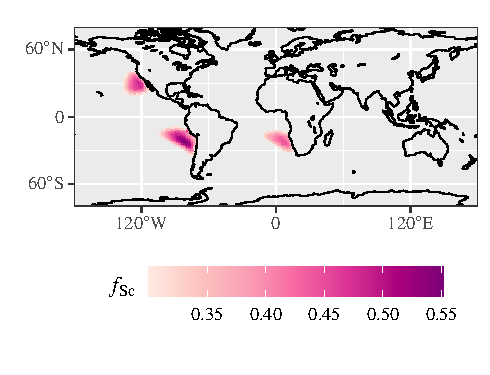
\includegraphics[width=8.3cm]{figure/fscu-1} 

}


\end{knitrout}
  \caption{Occurrence fraction $f_\text{Sc}$ of Sc conditions by the \citet{Medeiros2011}
    criteria in EAMv1, shown where $f_\text{Sc} > 0.3$ (NEP, southeast
    Pacific, southeast Atlantic Sc regions).}
  \label{fig:fscu}
\end{figure*}
%
\clearpage
%
\begin{figure*}[t]
  \centering
  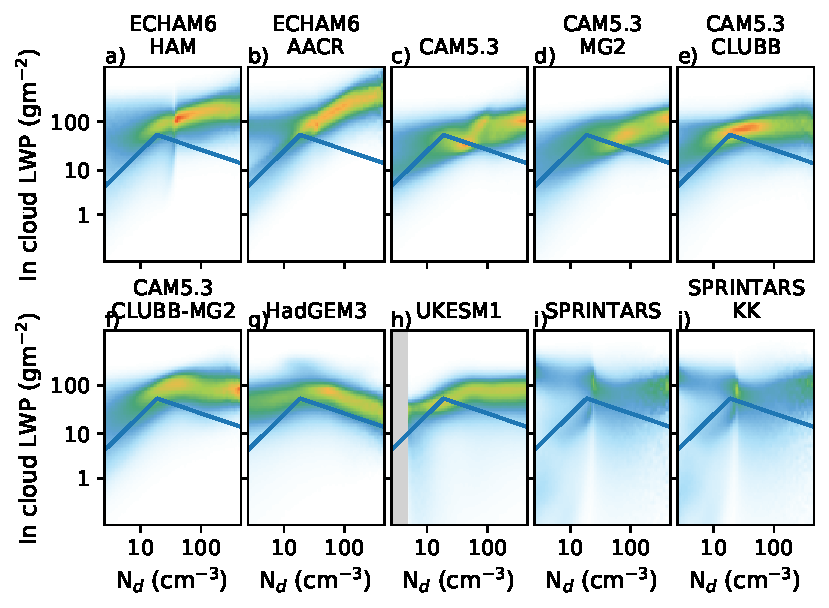
\includegraphics[width=12cm]{figure/aerocom.pdf}
  % <<aerocom-plot-heatmap>>=
  % @ 
  \caption{AeroCom IND3 state-of-the-art models' \nd--\lwp{} relationship.
    The satellite inverted v relationship \citep{Gryspeerdt2019} is
    indicated by the solid line.}
  \label{fig:ind3}
\end{figure*}
%
\clearpage
%

\begin{figure*}[t]
  \centering


\begin{knitrout}
\definecolor{shadecolor}{rgb}{0.969, 0.969, 0.969}\color{fgcolor}

{\centering 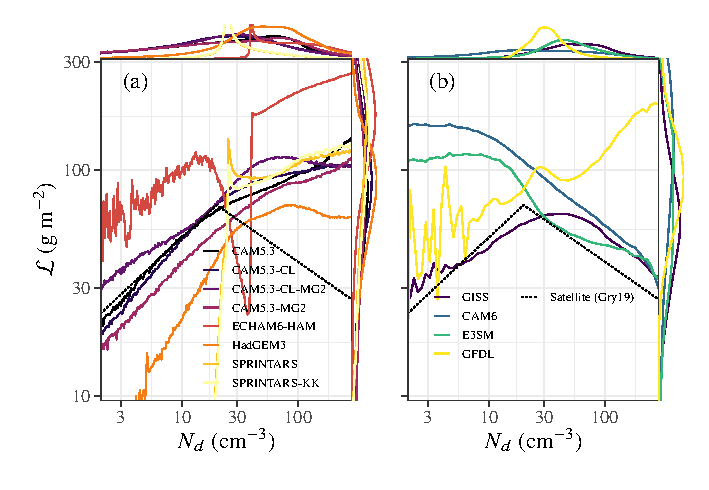
\includegraphics[width=12cm]{figure/multimodel-pd-plot-print-1} 

}


\end{knitrout}
  \caption{AeroCom IND3 state-of-the-art models' marginal distributions of \nd{} and
    \lwp{} and \nd--\lwp{} relationship (a) compared
    to the CMIP6-era state-of-the-art models' \nd--\lwp{} relationship (b).  The
    satellite inverted v relationship \citep{Gryspeerdt2019} is indicated by
    the dotted line.  Three of the four CMIP6 models examined are qualitatively
    similar to the satellite result in the sense that the \nd--\lwp{}
    correlation turns negative at moderate \nd{}.}
  \label{fig:aerocom-cms-line-plot}
\end{figure*}
%
\clearpage
%

\begin{figure}
  \centering
\begin{knitrout}
\definecolor{shadecolor}{rgb}{0.969, 0.969, 0.969}\color{fgcolor}

{\centering 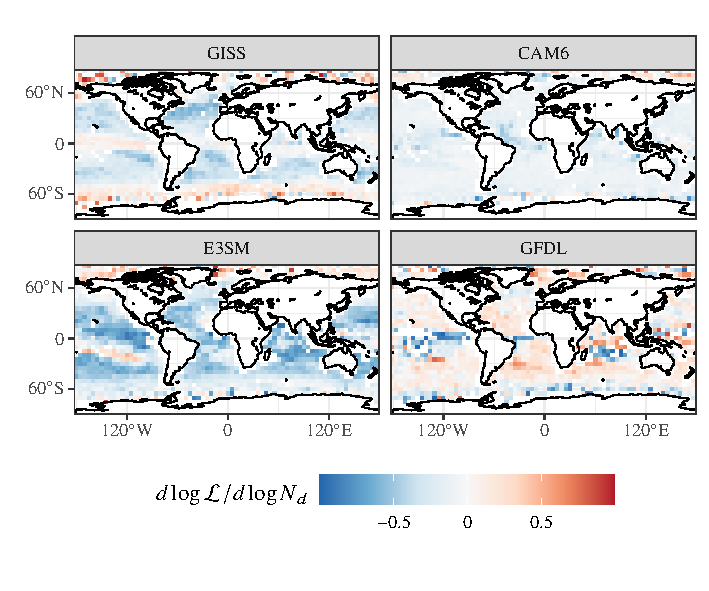
\includegraphics[width=12cm]{figure/multimodel-lon-lat-susc-plot-1} 

}


\end{knitrout}
  \caption{Geographic distribution of $d\log\lwp/d\log\nd$.  Model output is aggregated to $5\degree\times 5\degree$ latitude--longitude boxes before calculating linear regression slopes of $\log\lwp$ against $\log\nd$.}
  \label{fig:multimodel-lon-lat-susc}
\end{figure}
%
\clearpage
%
%
% \begin{figure*}[t]
%   \centering
%   <<multimodel-pd-plot>>=
%   @ 
%   \caption{CMIP6-era state of the art \nd--\lwp{} correlation \hl{only show PD,
%       then have separate figure for PD+PI lines in E3SM and GISS, justified by
%       their being two different-physics models that show a negative
%       correlation} \jmcomment{Combine Figs.~\ref{fig:aerocom-line-plot} and
%       \ref{fig:cms} into one figure with two panels}}
%   \label{fig:cms}
% \end{figure*}
%
% \clearpage
%
\begin{figure*}[t]
  \centering
  % <<multimodel-selected-ecdf-lwp>>=
  % @

\begin{knitrout}
\definecolor{shadecolor}{rgb}{0.969, 0.969, 0.969}\color{fgcolor}

{\centering 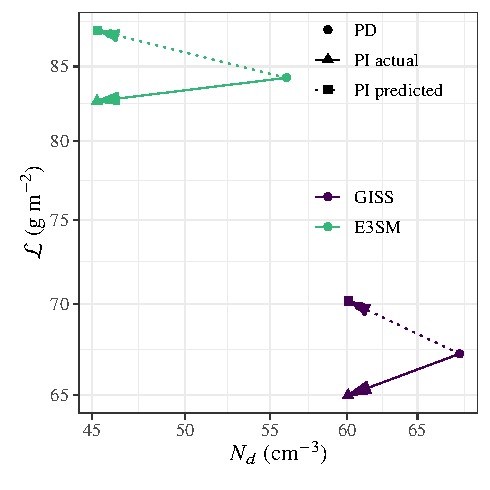
\includegraphics[width=8.3cm]{figure/multimodel-delta-pred-actual-plot-1} 

}


\end{knitrout}
  \caption{PI--PD \lwp{} change from the causal experiment (solid arrow)
    contrasted with the change predicted from the PD internal variability
    (dashed arrow).  The mean $\log\lwp$ as a function of $\log\nd$ from the PD
    model run (Fig.~\ref{fig:aerocom-cms-line-plot}) is used to predict PI mean $\log\lwp$ from the PI $\log\nd$
    distribution.
    Even though the PD \nd--\lwp{} correlation is negative,
    $\lwp_\text{PD} > \lwp_\text{PI}$.}
  \label{fig:pdpi-causal-pred}
\end{figure*}
%
\clearpage
%
\begin{figure*}[t]
  \centering

\begin{knitrout}
\definecolor{shadecolor}{rgb}{0.969, 0.969, 0.969}\color{fgcolor}

{\centering 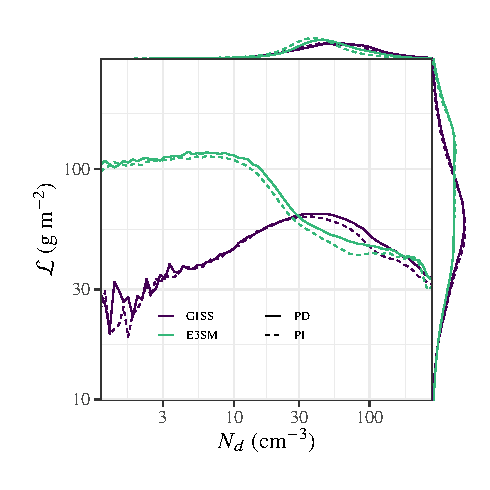
\includegraphics[width=8.3cm]{figure/multimodel-selected-pd-pi-plot-print-1} 

}


\end{knitrout}
  \caption{PD (solid) and PI (dashed) \nd{} and \lwp{} marginal distributions
    and \nd--\lwp{} correlation in two GCMs with
    unrelated turbulence schemes.  The \nd--\lwp{} relationship based on
    internal variability within one climate state is not universal across the
    states.}
  \label{fig:cms-selected}
\end{figure*}
%
\clearpage
%
% \begin{figure*}[t]
%   \centering
%   <<multimodel-selected-plot-lwp>>=
%   @ 
%   \caption{Even when the \nd--\lwp{} correlation is negative,
%     $\lwp_\text{PD} > \lwp_\text{PI}$}
%   \label{fig:pdpi}
% \end{figure*}
%
% \clearpage
%

% <<e3sm-precip-exps-setup>>=
% @
\begin{figure*}[t]
  \centering
\begin{knitrout}
\definecolor{shadecolor}{rgb}{0.969, 0.969, 0.969}\color{fgcolor}

{\centering 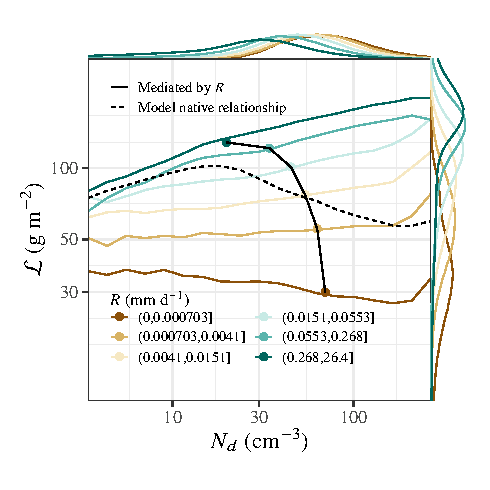
\includegraphics[width=8.3cm]{figure/precip-lwp-cdnc-1} 

}


\end{knitrout}
  \caption{Precipitation-stratified \nd{} and \lwp{} marginal distributions
    and \nd--\lwp{} relationships (colored lines).  The dashed black line shows
    the unstratified \nd--\lwp{} relationship.  The solid black line connects
    the mean $(\nd,\lwp)$ in each precipitation sextile (colored dots).
    Binning by precipitation intensity exposes a precipitation-mediated 
    negative \nd--\lwp{} covariability with a much steeper slope than the overall
    \nd--\lwp{} correlation, even though the \nd--\lwp{} correlation within all but the
    least precipitating sextile is positive.}
  \label{fig:precip}
\end{figure*}
%
\clearpage
%
\begin{figure*}
  \centering

  
\begin{knitrout}
\definecolor{shadecolor}{rgb}{0.969, 0.969, 0.969}\color{fgcolor}

{\centering 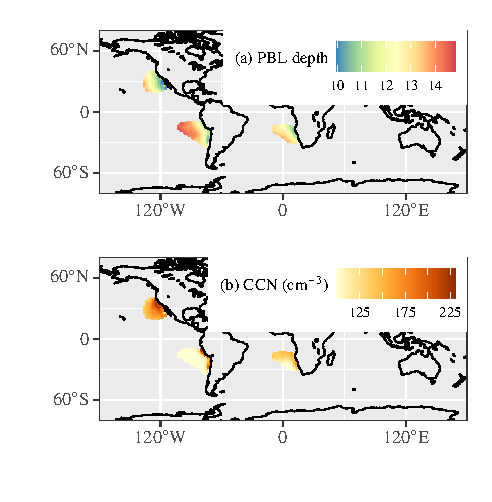
\includegraphics[width=8.3cm]{figure/covariability-space-plot-1} 

}


\end{knitrout}
  \caption{Within the Sc regime, synoptic-scale meteorology results in strong
    spatial covariability of (a) PBL depth (measured in model levels) and (b)
    CCN concentration at 0.2\% supersaturation averaged over the depth of the
    PBL.  Both of these variables are functions of airmass continentality.}
  \label{fig:covariability-space}
\end{figure*}
%
\clearpage
%
% \begin{figure*}
%   \centering
%   <<pbl-met-geo>>=
%   df.ccn %>%
%       filter(is.scu) %>%
%       filter(jk.pbl %in% 9:15) %>%
%       group_by(lon, lat) %>%
%       summarize(jk.pbl = round(median(jk.pbl))) %>%
%       ungroup() %>%
%       mutate(lon = ifelse(lon > 180, lon - 360, lon)) %>%
%       ggplot(aes(lon, lat, col = factor(jk.pbl, levels = 10:15))) +
%       geom_point(size = 1.5) +
%       geom_world_polygon(highres = FALSE) +
%       scale_x_geo() +
%       scale_y_geo() +
%       coord_fixed(1, c(-150, -115), c(14, 36)) +
%       scale_color_brewer("$k - k_\\text{pbl}$", palette = "Spectral", drop = FALSE,
%                          guide = guide_legend()) +
%       theme(axis.title.x = element_blank()) +
%       theme(legend.position = "bottom", legend.direction = "horizontal")

%   @
%   \caption{\jmcomment{Insert figure showing PBL depth increases further
%       offshore} \jmcomment{Note that points over land are excluded in aggregates}}
%   \label{fig:continentality-pblh}
% \end{figure*}
% %
% \clearpage
% %
\begin{figure*}[t]
  \centering

\begin{knitrout}
\definecolor{shadecolor}{rgb}{0.969, 0.969, 0.969}\color{fgcolor}

{\centering 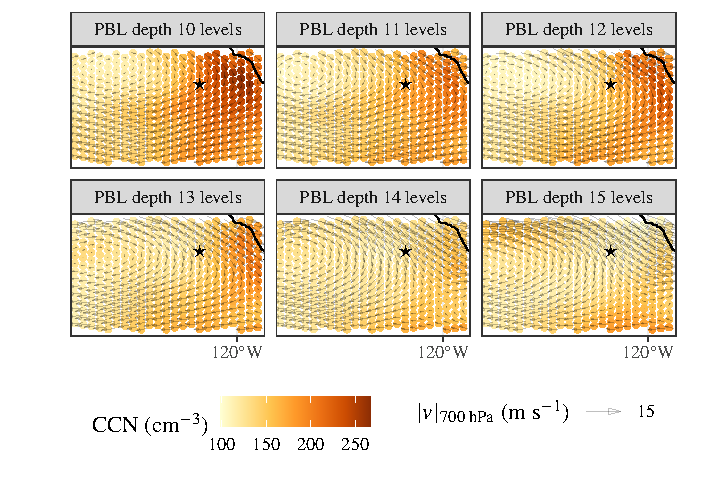
\includegraphics[width=12cm]{figure/e3sm-ccn-met-plot-1} 

}


\end{knitrout}
  \caption{Within the Sc regime, synoptic-scale meteorology
    results in strong temporal covariability between CCN
    and PBL depth.   This is exemplified by the NEP;
    the Southern
    California Bight is depicted in top right corner.  The star indicates
    the grid point
    with the highest occurrence fraction of Sc
    conditions according to the criteria of \citet{Medeiros2011}. (Aggregates exclude points over land.)} 
  \label{fig:covariability}
\end{figure*}
%
\clearpage
% 
\begin{figure*}[t]
  \centering
\begin{knitrout}
\definecolor{shadecolor}{rgb}{0.969, 0.969, 0.969}\color{fgcolor}

{\centering 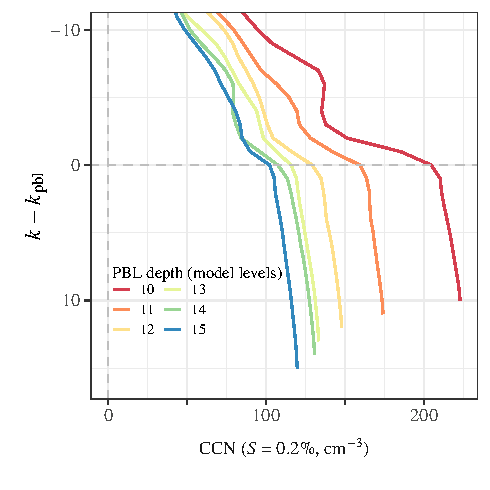
\includegraphics[width=8.3cm]{figure/profiles-ccn-1} 

}


\end{knitrout}
  \caption{Temporal and regional-mean CCN concentration profiles in the NEP Sc
    region stratified by PBL depth.  Within the Sc regime, CCN is strongly
    sorted by PBL depth, illustrating the strong covariability between PBL
    thermodynamic structure and aerosol advection.
    %% df.profiles.jk.pbl %>% filter(precc == 0) %$% quantile(jk.pbl, c(0.05, 0.95))    
    The central 90\% of the PBL depth range (between 10 and 15 model levels,
    corresponding approximately to between 750--1400~m) is shown to avoid outliers in the
    low-statistics PBL depth bins.  The PBL depth is measured in units of model
    levels $k$, with $k$ decreasing downward from the level of the PBL-capping
    inversion $k_\text{pbl}$ to the model level closest to the surface ($k=72$
    in EAMv1).}
  % <<table-level-heights>>=
  % df.profiles.nep %>%
  %     filter(is.na(ilev)) %>%
  %     group_by(time) %>%
  %     mutate(jk = 1:72) %>%
  %     ungroup() %>%
  %     group_by(jk) %>%
  %     summarize(lev.sd = sd(lev), lev = mean(lev), ## note this is just the hybrid coeff assuming ps = 1000
  %               z.sd = sd(z3), z = mean(z3)) %>%
  %     ungroup() %>%
  %     mutate(jk = 73 - jk) %>%
  %     print(n = 100)
  % @
  \label{fig:ccnprof}
\end{figure*}
%
\clearpage
%
\begin{figure*}[t]
  \centering
\begin{knitrout}
\definecolor{shadecolor}{rgb}{0.969, 0.969, 0.969}\color{fgcolor}

{\centering 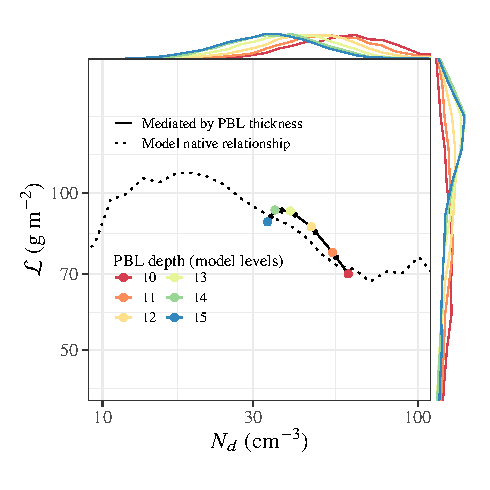
\includegraphics[width=8.3cm]{figure/e3sm-pblh-plot-1} 

}


\end{knitrout}
  \caption{Within the Sc regime, PBL depth--CCN covariability leads to a
    negative \nd--\lwp{} correlation with slope similar to the overall
    \nd--\lwp{} correlation.  The dashed black line shows
    the \nd--\lwp{} relationship not stratified by PBL depth.  The solid black line connects
    the mean $(\nd,\lwp)$ at each PBL depth (colored dots).  The central 90\% of the PBL depth range (between 10 and 15 model levels) is shown to avoid outliers in the
    low-statistics PBL depth bins.}
  \label{fig:pblh}
\end{figure*}
%
\clearpage
%
\begin{figure*}[t]
  \centering
\begin{knitrout}
\definecolor{shadecolor}{rgb}{0.969, 0.969, 0.969}\color{fgcolor}

{\centering 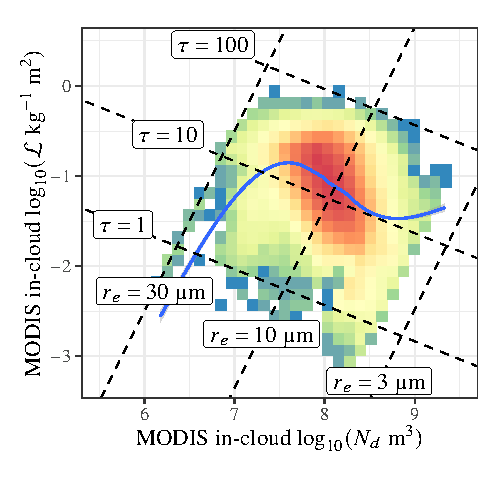
\includegraphics[width=8.3cm]{figure/cosp-tau-re-plot-1} 

}


\end{knitrout}
  \caption{Joint probability distribution of E3SM MODIS-simulated \lwp{} and
    \nd{}.  Isolines of $r_e$ and $\tau$, from which adiabatic \nd{} and \lwp{}
    are retrieved, are overlaid.  The mean $\log\lwp$ as a function of $\log
    \nd$ is shown as a blue line.  Because the model imposes a rectangular limit
    on $r_e$ and $\tau$, the \nd--\lwp{} phase space has parallelogram-shaped
    boundaries.  At least part of the rise, fall, and repeated rise of \lwp{} as
    a function of \nd{} (blue line) is due to these phase-space boundaries cutting off the upper and lower parts of the \lwp{} distribution.}
  \label{fig:cosp}
\end{figure*}
%
\clearpage
%
%%% TABLES
%%%
%%% The different columns must be seperated with a & command and should
%%% end with \\ to identify the column brake.
%
%%% ONE-COLUMN TABLE
%
%%t
%\begin{table}[t]
%\caption{TEXT}
%\begin{tabular}{column = lcr}
%\tophline
%
%\middlehline
%
%\bottomhline
%\end{tabular}
%\belowtable{} % Table Footnotes
%\end{table}
%
%%% TWO-COLUMN TABLE
%
%%t
\begin{table*}[t]
  \caption{GCM experiments used in this analysis.}
  \label{tab:exp}
  \begin{tabular}{llll}
    \tophline
    Experiment & Emissions & Cloud selection & Duration \\
    \middlehline
    Multimodel PD & Present-day & Global overcast & 2010, nudged \\
    Multimodel PI & Preindustrial & Global overcast & 2011, nudged \\
    E3SM + COSP simulator & Present-day & NEP Sc regime & 2010, nudged \\
    E3SM precip & Present-day & Sc regime & 2010--2014, nudged \\
    \bottomhline
  \belowtable{} % Table Footnotes
  \end{tabular}
\end{table*}
%
\clearpage
%
% \begin{table*}[t]
%   \caption{TEXT}
%   \label{tab:occ}
%   \begin{tabular}{lcr}
%     \tophline
    
%     \middlehline
    
%     \bottomhline

%     <<occurrence-table, results='asis'>>=

%     @ 
%   \end{tabular}
%   \belowtable{} % Table Footnotes
% \end{table*}
%
%%% LANDSCAPE TABLE
%
%%t
%\begin{sidewaystable*}[t]
%\caption{TEXT}
%\begin{tabular}{column = lcr}
%\tophline
%
%\middlehline
%
%\bottomhline
%\end{tabular}
%\belowtable{} % Table Footnotes
%\end{sidewaystable*}
%
%
%%% MATHEMATICAL EXPRESSIONS
%
%%% All papers typeset by Copernicus Publications follow the math typesetting regulations
%%% given by the IUPAC Green Book (IUPAC: Quantities, Units and Symbols in Physical Chemistry,
%%% 2nd Edn., Blackwell Science, available at: http://old.iupac.org/publications/books/gbook/green_book_2ed.pdf, 1993).
%%%
%%% Physical quantities/variables are typeset in italic font (t for time, T for Temperature)
%%% Indices which are not defined are typeset in italic font (x, y, z, a, b, c)
%%% Items/objects which are defined are typeset in roman font (Car A, Car B)
%%% Descriptions/specifications which are defined by itself are typeset in roman font (abs, rel, ref, tot, net, ice)
%%% Abbreviations from 2 letters are typeset in roman font (RH, LAI)
%%% Vectors are identified in bold italic font using \vec{x}
%%% Matrices are identified in bold roman font
%%% Multiplication signs are typeset using the LaTeX commands \times (for vector products, grids, and exponential notations) or \cdot
%%% The character * should not be applied as mutliplication sign
%
%
%%% EQUATIONS
%
%%% Single-row equation
%
%\begin{equation}
%
%\end{equation}
%
%%% Multiline equation
%
%\begin{align}
%& 3 + 5 = 8\\
%& 3 + 5 = 8\\
%& 3 + 5 = 8
%\end{align}
%
%
%%% MATRICES
%
%\begin{matrix}
%x & y & z\\
%x & y & z\\
%x & y & z\\
%\end{matrix}
%
%
%%% ALGORITHM
%
%\begin{algorithm}
%\caption{...}
%\label{a1}
%\begin{algorithmic}
%...
%\end{algorithmic}
%\end{algorithm}
%
%
%%% CHEMICAL FORMULAS AND REACTIONS
%
%%% For formulas embedded in the text, please use \chem{}
%
%%% The reaction environment creates labels including the letter R, i.e. (R1), (R2), etc.
%
%\begin{reaction}
%%% \rightarrow should be used for normal (one-way) chemical reactions
%%% \rightleftharpoons should be used for equilibria
%%% \leftrightarrow should be used for resonance structures
%\end{reaction}
%
%
%%% PHYSICAL UNITS
%%%
%%% Please use \unit{} and apply the exponential notation

\appendix
% \section{}    %% Appendix A

% \subsection{}     %% Appendix A1, A2, etc.


% %% Regarding figures and tables in appendices, the following two options are possible depending on your general handling of figures and tables in the manuscript environment:

% %% Option 1: If you sorted all figures and tables into the sections of the text, please also sort the appendix figures and appendix tables into the respective appendix sections.
% %% They will be correctly named automatically.

% %% Option 2: If you put all figures after the reference list, please insert appendix tables and figures after the normal tables and figures.
% %% To rename them correctly to A1, A2, etc., please add the following commands in front of them:

\appendixfigures  %% needs to be added in front of appendix figures

% \begin{figure}
%   \centering
%   <<multimodel-plot-lcc-0.1>>=
%   @ 
%   <<multimodel-plot-lcc-0.1-print>>=
%   ggplot.multimodel.lcc.0.1 + labs_nd_lwp_conventional()
%   @ 
%   \caption{Dependence of \nd--\lwp{} relationship on cloud fraction threshold}
%   \label{fig:multimodel-fc}
% \end{figure}

% \appendixtables   %% needs to be added in front of appendix tables

% %% Please add \clearpage between each table and/or figure. Further guidelines on figures and tables can be found below.

\noappendix       %% use this to mark the end of the appendix section. Otherwise the figures might be numbered incorrectly (e.g. 10 instead of 1).


\end{document}
